  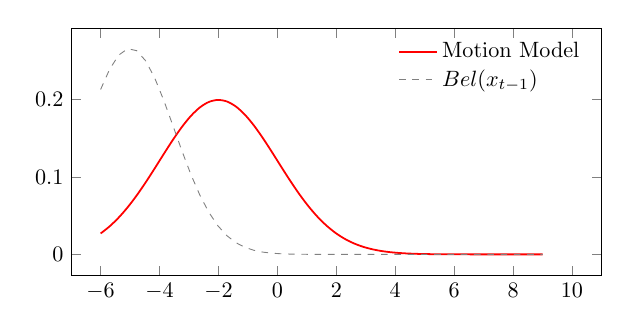
\begin{tikzpicture}[
    declare function={
      normalpdf(\x,\mu,\sigma)=
      (2*3.1415*\sigma^2)^(-0.5)*exp(-(\x-\mu)^2/(2*\sigma^2));
    },
    hplot/.style={ycomb, mark=o, dashed}, ,scale=0.8]
  
    \begin{axis}[
      width=10cm, height=5.5cm,
      samples=50,
      legend style={draw=none, fill=none},
      domain=-6:9,
      legend cell align=left,
      xmin=-7, xmax=11]
  
      \addplot [smooth, thick, red] {normalpdf(x,-2,2)} node[] {};
      \addplot [dashed, gray]       {normalpdf(x,-5,1.5)} node[] {};
      \legend{Motion Model, $\text{Bel}(x_{t-1})$};
    \end{axis}
  \end{tikzpicture}
  \pausar
  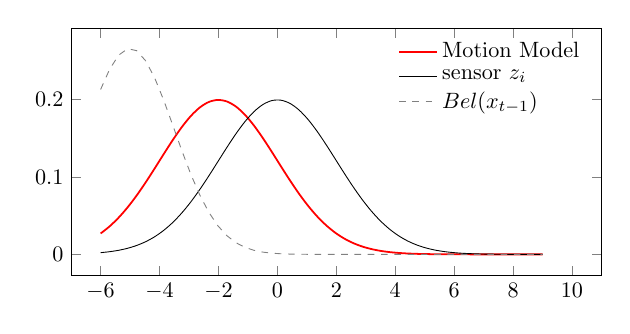
\begin{tikzpicture}[
    declare function={
      normalpdf(\x,\mu,\sigma)=
      (2*3.1415*\sigma^2)^(-0.5)*exp(-(\x-\mu)^2/(2*\sigma^2));
    },
    hplot/.style={ycomb, mark=o, dashed}, ,scale=0.8]
  
    \begin{axis}[
      width=10cm, height=5.5cm,
      samples=50,
      legend style={draw=none, fill=none},
      domain=-6:9,
      legend cell align=left,
      xmin=-7, xmax=11]
  
      \addplot [smooth, thick, red] {normalpdf(x,-2,2)} node[] {};
      \addplot [smooth, black] {normalpdf(x,0,2)} node[] {};
      \addplot [dashed, gray]       {normalpdf(x,-5,1.5)} node[] {};
      \legend{Motion Model, sensor $z_i$, $\text{Bel}(x_{t-1})$};
    \end{axis}
  \end{tikzpicture}

  \pausar

\begin{columns}

  \begin{column}{0.5\textwidth}

    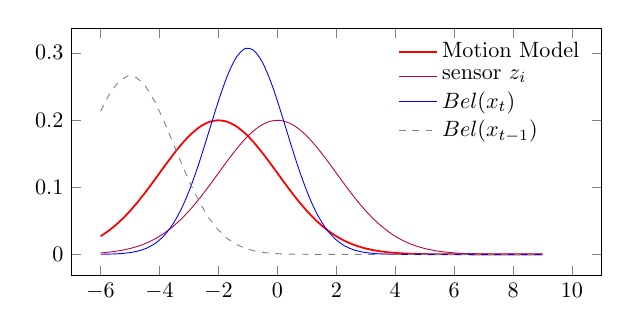
\begin{tikzpicture}[
      declare function={
        normalpdf(\x,\mu,\sigma)=
        (2*3.1415*\sigma^2)^(-0.5)*exp(-(\x-\mu)^2/(2*\sigma^2));
      },
      hplot/.style={ycomb, mark=o, dashed}, ,scale=0.8]
    
      \begin{axis}[
        width=10cm, height=5.5cm,
        samples=50,
        legend style={draw=none, fill=none},
        domain=-6:9,
        legend cell align=left,
        xmin=-7, xmax=11]
    
        \addplot [smooth, thick, red] {normalpdf(x,-2,2)} node[] {};
        \addplot [smooth, purple]      {normalpdf(x,0,2)} node[] {};
        \addplot [smooth, blue]       {normalpdf(x,-1,1.3)} node[] {};
        \addplot [dashed, gray]       {normalpdf(x,-5,1.5)} node[] {};
        \legend{Motion Model, sensor $z_i$, $\text{Bel}(x_t)$, $\text{Bel}(x_{t-1})$};
      \end{axis}
    \end{tikzpicture}
  \end{column}

  \pausar

  \begin{column}{0.5\textwidth}
      How can the solution for the blue graph be found??

      \pausar
        $\textcolor{blue}{\text{Bel}(x_t)} =\eta \textcolor{purple}{P(z_t|x_t)}\displaystyle\int \textcolor{red}{P(x_t| u_t,x_{t-1})}\textcolor{gray}{\text{Bel}(x_{t-1})}\text{d}x_{t-1}$

        onde:
        \begin{tabular}{l  l}
          $z_t$: & state observed in time $t$\\ 
          $u_t$: & action in time $t$\\
          $x_t$: & system state in em $t$        
        \end{tabular}
    
  \end{column}
\end{columns}
